\documentclass[pdflatex,a4paper,sn-nature]{sn-jnl}
% Compact manuscript layout; publisher class remains byte-for-byte unchanged.
\usepackage{etoolbox}
\geometry{reset,a4paper,left=20mm,right=20mm,top=16mm,bottom=16mm,headsep=3mm,footskip=9mm}
\makeatletter
\patchcmd{\@maketitle}{\vskip21pt}{\vskip0pt}{}{}
\patchcmd{\@maketitle}{\vskip20pt}{\vskip6pt}{}{}
\patchcmd{\@maketitle}{\vskip20pt}{\vskip10pt}{}{}
\patchcmd{\@maketitle}{\vskip24pt}{\vskip6pt}{}{}
\patchcmd{\@maketitle}{\vskip24pt}{\vskip6pt}{}{}
\patchcmd{\@maketitle}{\vskip36pt}{\vskip12pt}{}{}
\makeatother
\setcounter{topnumber}{3}
\setcounter{bottomnumber}{2}
\setcounter{totalnumber}{4}
\renewcommand{\topfraction}{.9}
\renewcommand{\bottomfraction}{.8}
\renewcommand{\textfraction}{.08}
\renewcommand{\floatpagefraction}{.75}
\setlength{\textfloatsep}{12pt plus 2pt minus 2pt}
\setlength{\floatsep}{10pt plus 2pt minus 2pt}

\makeatletter
\setlength{\@fptop}{0pt}
\setlength{\@fpsep}{14pt}
\setlength{\@fpbot}{0pt plus 1fil}
\AtBeginDocument{\renewcommand{\Titlefont}{\normalfont\bfseries\fontsize{19}{23}\selectfont\raggedright}}
\makeatother
\makeatletter
\AtBeginDocument{\renewcommand{\bibfont}{\normalfont\fontsize{9}{10.5}\selectfont}\setlength{\bibsep}{2pt}}
\makeatother

\setcitestyle{square}
\usepackage{amsmath,amssymb,booktabs,graphicx,placeins}
\renewcommand{\thefigure}{S\arabic{figure}}
\renewcommand{\thetable}{S\arabic{table}}
\makeatletter
\def\fnum@figure{Supplementary Fig.\ \thefigure}
\def\fnum@table{Supplementary Table\ \thetable}
\makeatother
\raggedbottom
\begin{document}
\title[Supplementary information]{Supplementary Information for: Pasture biomass estimation using transferred I-JEPA and DINOv3 representations}
\author*[1]{\fnm{Chandrakala G} \sur{Raju}}\email{chandrakalagraju.ise@bmsce.ac.in}
\author[1]{\fnm{Megh Mayur} \sur{M R}}\email{meghmayur.is23@bmsce.ac.in}
\author[1]{\fnm{Mohd. Viquaruddin} \sur{Anas}}\email{mohdviquaruddin.is23@bmsce.ac.in}
\author[1]{\fnm{Karthik} \sur{N H}}\email{karthiknh.is23@bmsce.ac.in}
\affil[1]{\orgdiv{Department of Information Science and Engineering}, \orgname{B.M.S. College of Engineering}, \orgaddress{\street{Bull Temple Road}, \city{Bengaluru}, \postcode{560019}, \state{Karnataka}, \country{India}}}
\maketitle
\noindent\textit{Corresponding author ORCID:} \url{https://orcid.org/0000-0002-5577-0024}\par

\section*{Supplementary Methods}
The accompanying local evidence archive SR-release-r7-authors-2026-10-11 contains saved predictions, the 357-image fold manifest, verification scripts and SHA-256 checksums. It provides reviewer-accessible arithmetic reproduction, not a public code or checkpoint release.

\subsection*{Fold membership and score interpretation}
The 105-photograph analysis pools validation predictions from folds 0 and 1. Fold 0 contains 308 training and 49 validation photographs; fold 1 contains 301 training and 56 validation photographs. The validation images are distinct across these folds, and the groups correspond to nine recorded acquisition dates. These are repeated development folds. The separate block-augmentation comparison covers 167 photographs from folds 0--2 and 14 dates. Neither evaluation is a full out-of-fold evaluation of all 357 photographs, a protected confirmation set, or a competition score. Confidence intervals reported in the main text resample acquisition-date groups while holding saved model predictions fixed.

\subsection*{Derived predictions and target metric}
All models predict nonnegative Green, Clover, and Dead primitive masses and derive GDM and Total by summation. The primary score is one weighted $R^2$ computed on the pooled five-target prediction matrix. The weights sum to one and are applied to squared residuals and squared deviations around one weighted mean over pooled observations. Consequently, a weighted average of target-specific $R^2$ values does not equal the globally weighted $R^2$. Raw gram units are preserved for MAE and RMSE. No log-transformed objective or log-space score is used in the reported frozen-head and DINOv3 depth comparisons.

\section*{Supplementary Results}
\subsection*{Conditional paired date-group comparisons}
The paired comparisons below use 10,000 bootstrap resamples and seed 42. The intervals condition on the listed development predictions and nine observed date groups; they do not account for training-seed or model-selection variation.

\begin{table}[ht]
\centering
\caption{Primary paired differences in raw global weighted $R^2$ on the 105-photograph development set.}
\begin{tabular}{lrr}
\toprule Comparison & Difference & Conditional 95\% interval \\
\midrule
Grass-adapted minus original I-JEPA & 0.039521 & [0.001930, 0.091947] \\
F2 minus F1 & $-0.001474$ & [$-0.004676$, 0.000041] \\
Predictor shuffle minus unshuffled & 0.007801 & [$-0.026260$, 0.043753] \\
DINOv3 D1 minus D0 & 0.013969 & [$-0.018280$, 0.046373] \\
DINOv3 D2 minus D1 & 0.000184 & [$-0.000098$, 0.000437] \\
Depth 4 minus depth 2 & $-0.004539$ & [$-0.008556$, $-0.000764$] \\
Depth 8 minus depth 2 & $-0.006705$ & [$-0.011834$, $-0.000076$] \\
\bottomrule
\end{tabular}
\label{tab:s1}
\end{table}

For the distinct 167-image permutation-augmentation study, the control scored 0.616304, $4\times4$ permutation scored 0.583541, and $10\times10$ permutation scored 0.565459. The respective differences from control were $-0.032763$ (95\% interval $[-0.070229,0.020309]$) and $-0.050845$ (interval $[-0.100372,0.013122]$), based on 14 date groups. These values must not be pooled with the two-fold comparisons above.

\subsection*{DINOv3 sensitivity examples}
The matched sensitivity analysis evaluated three fixed-seed, uniformly sampled photographs under each fold-one depth checkpoint. The maximum absolute difference between saved training-precision and CPU FP32 prediction across the nine cases was 2.4136734~g. Four gradient-ranked cells produced larger absolute Total-output changes than four randomly selected cells in six of nine cases. Thus, this small comparison was not uniformly favorable to gradient ranking. Individual examples, target vectors, selected cell indices, checkpoint hashes, and perturbation changes are retained in the accompanying machine-readable analysis artifacts. The examples are identified in the figure headers by photograph ID solely to document provenance; they are not independently sampled confirmation observations.

\subsection*{Historical context-readout provenance}
An earlier recorded development score of 0.83404 came from a separate DINOv3-L-backed JEPA-style context-readout lineage, not the official I-JEPA ViT-H/14. Original fold-table bytes are unavailable, so its original held-out membership remains unverified. It is excluded from the main performance comparisons. Historical sensitivity panels are omitted from this supplement; preserved project artifacts retain the diagnostics without treating them as independent validation.

\section*{Source target audit}
Across all 357 publicly labeled training images, exact-zero Clover and Dead counts were 135 and 40. In the held-out 105-image development subset they were 47 and one. Maximum GDM accounting residual was 0.0001~g; one Total residual exceeded 0.01~g (0.3088~g maximum) in the full set, and none exceeded that threshold in the development subset. Total medians were 40.3~g overall and 49.1~g in the 105-image subset. These differences describe the selected evaluation distribution, not an independently protected test population.
\section*{Original evidence versus replication}
The current analysis reuses preserved model predictions; no additional training was performed. F1/F2 and depth 2/4/8 predictions were recovered from their saved runs and independently rescored with exact image/date/fold/label alignment. F2 predictions exactly equal the depth-two prediction array. The historical 0.83404 record remains unverified for its original held-out split: checkpoint-family reconstruction and three examples do not reconstruct the missing historical fold table. It is excluded from the main results; a future execution would be a new replication, not recovery of that historical score.
\begin{table}[!htbp]
\centering\caption{Training-only constant baseline target errors on the same 105 pooled development photographs. Errors are grams; individual target $R^2$ is distinct from the globally weighted score.}
\begin{tabular}{llrrr}\toprule Baseline & Target & MAE & RMSE & $R^2$ \\
\midrule
Target means & Green & 23.93 & 34.12 & $-0.0772$ \\
Target means & Dead & 10.42 & 14.51 & $-0.0753$ \\
Target means & Clover & 9.11 & 13.55 & $-0.0854$ \\
Target means & GDM & 22.99 & 32.60 & $-0.1026$ \\
Target means & Total & 27.07 & 37.67 & $-0.1509$ \\
Primitive means & Green & 23.93 & 34.12 & $-0.0772$ \\
Primitive means & Dead & 10.42 & 14.51 & $-0.0753$ \\
Primitive means & Clover & 9.11 & 13.55 & $-0.0854$ \\
Primitive means & GDM & 22.99 & 32.60 & $-0.1026$ \\
Primitive means & Total & 27.07 & 37.67 & $-0.1509$ \\
\bottomrule\end{tabular}
\label{tab:s2}
\end{table}
\section*{Training-only constants and date influence}
Five-target and physically consistent training-mean constants scored 0.1440996 and 0.1441102, respectively. Full target errors and each fold's constants, training IDs and disjoint dates are in the accompanying CSV/JSON artifacts. No validation label was used to fit either baseline. The nine leave-one-date-out F2--F1 differences range from $-0.002380$ to $-0.000984$; F4--F2 from $-0.006312$ to $-0.002385$; F8--F2 from $-0.008625$ to $-0.003534$. All are negative. Per-date image counts and errors are supplied without interpreting dates as independently verified sites.
\section*{Precision and contribution arithmetic}
The maps use CPU FP32. Across nine model--image cases, absolute Total discrepancies from saved GPU predictions have a minimum, median and maximum of 0.0812, 0.8301 and 2.4137~g; relative discrepancies are 0.253\%, 1.974\% and 7.107\%, respectively, using saved prediction as denominator. All 45 target predictions differ by a nonzero amount. Actual GPU heatmap stability has not been tested. Displayed contribution proxies divide the raw head outputs by 128; the sum reconstructs the CPU prediction with maximum observed error of $1.53\times10^{-5}$ g. This is an arithmetic check, not validation of local biomass.

\FloatBarrier
\begin{figure}[!htbp]
\centering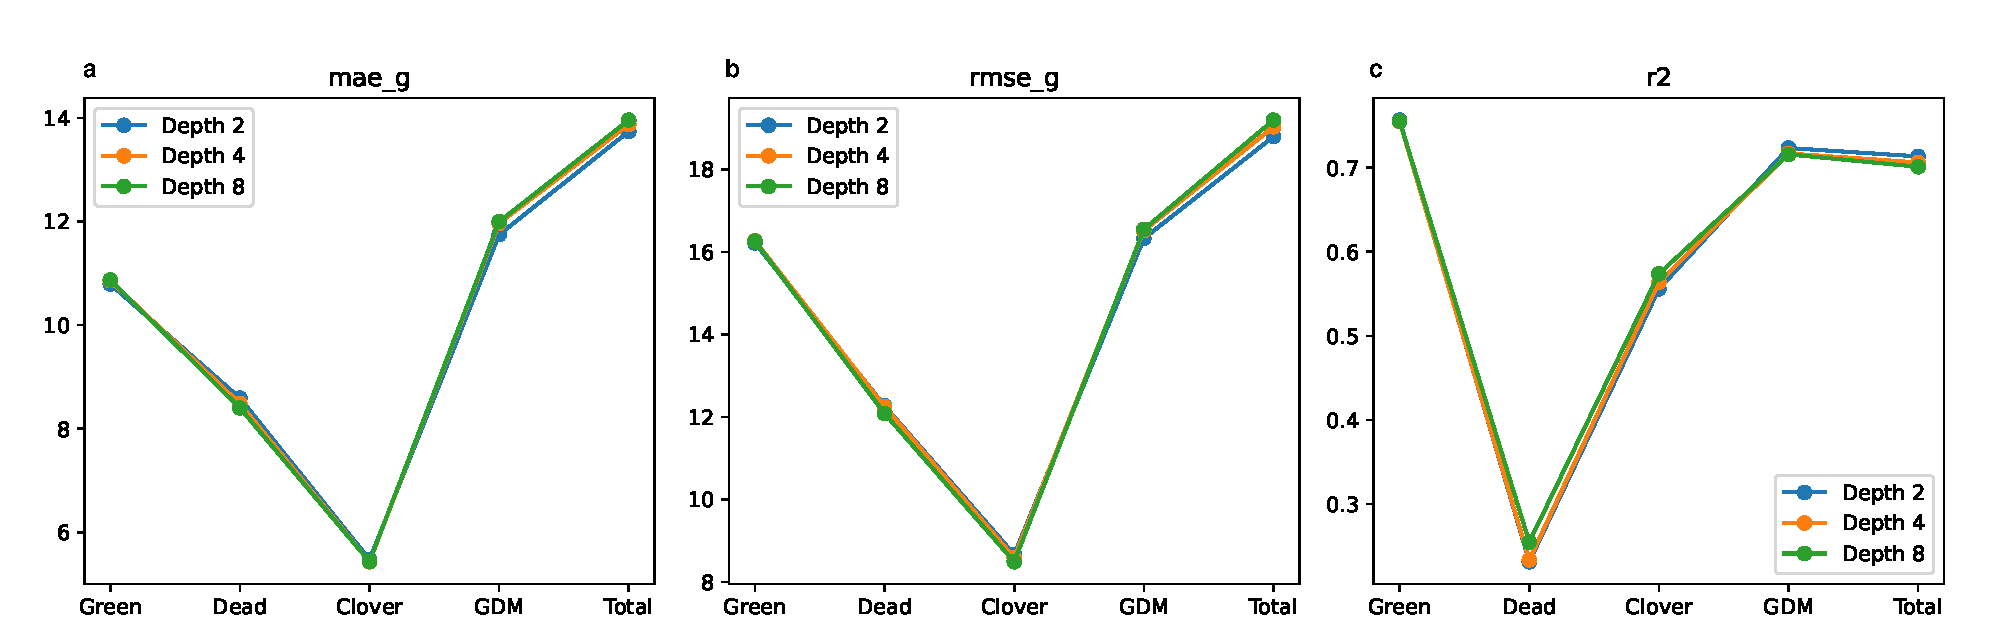
\includegraphics[width=\linewidth,height=.62\textheight,keepaspectratio]{figures/depth_per_target_metrics.pdf}
\caption{Per-target metrics for the two-, four- and eight-block models.}
\label{fig:s1}
\end{figure}
\begin{figure}[!htbp]
\centering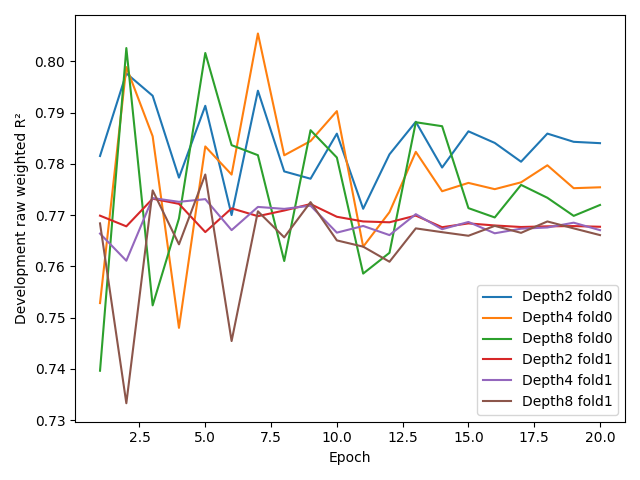
\includegraphics[width=\linewidth,height=.62\textheight,keepaspectratio]{figures/depth__depth_training_curves.png}
\caption{Per-epoch development weighted R² during supervised continuation. Checkpoint selection uses the fixed final epoch.}
\label{fig:s2}
\end{figure}
\begin{figure}[!htbp]
\centering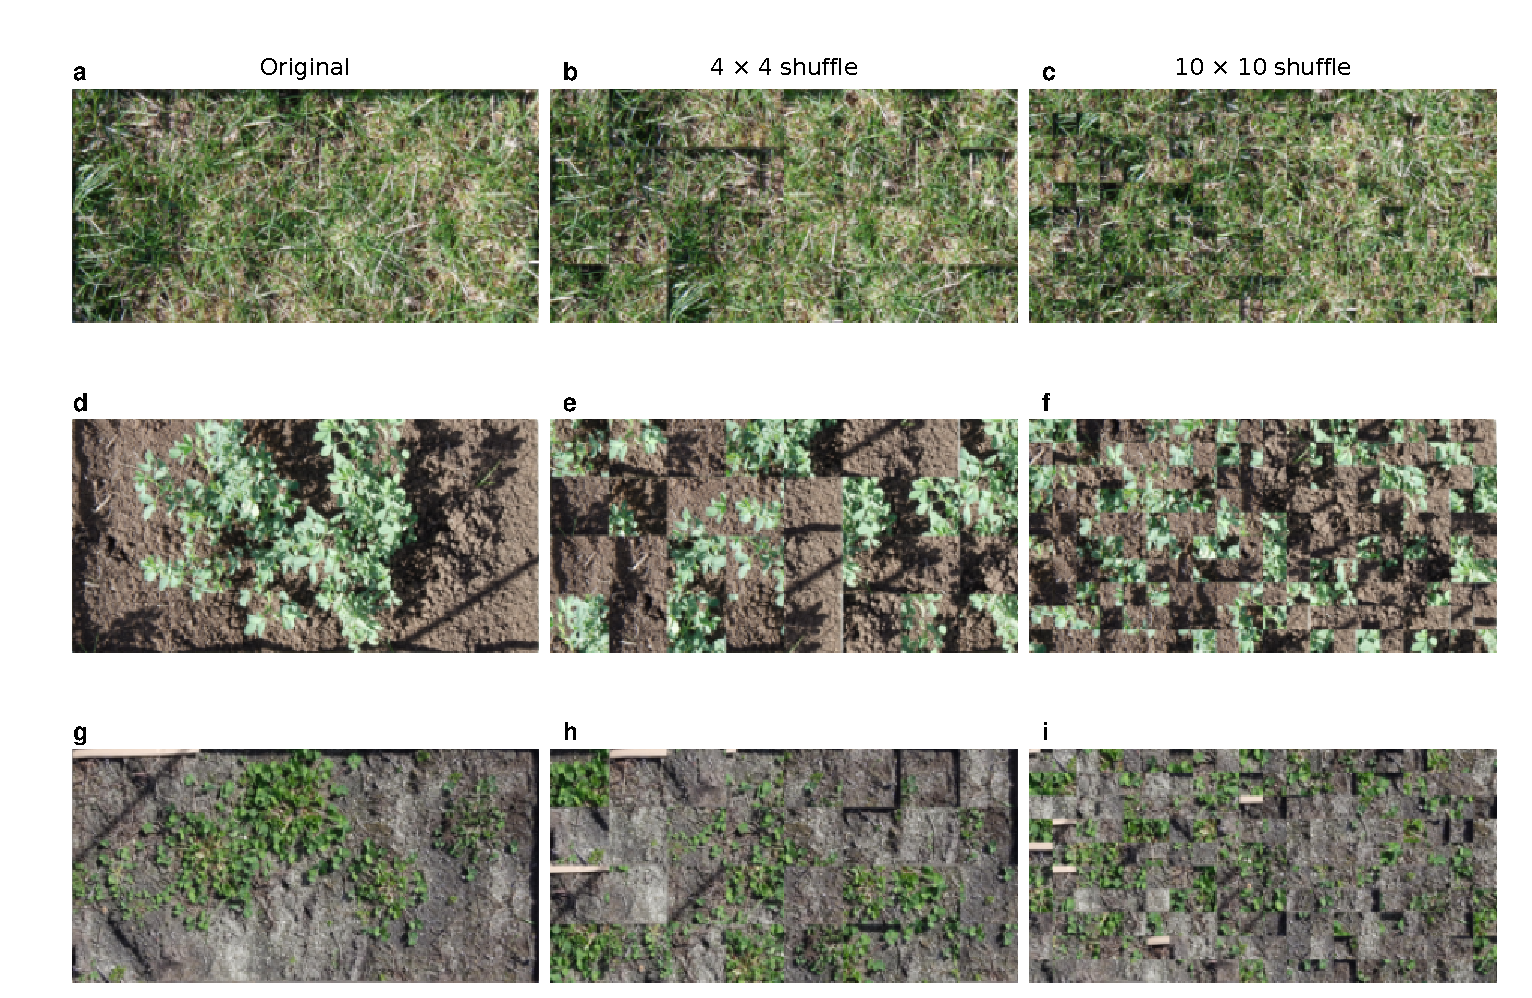
\includegraphics[width=\linewidth,height=.62\textheight,keepaspectratio]{figures/permutation_examples.pdf}
\caption{Original photographs and within-image spatial permutations for IDs ID1011485656, ID1012260530 and ID1025234388. Each square half is shuffled independently with the saved deterministic seeds. These are augmented views, not additional labeled photographs.}
\label{fig:s3}
\end{figure}
\begin{figure}[!htbp]
\centering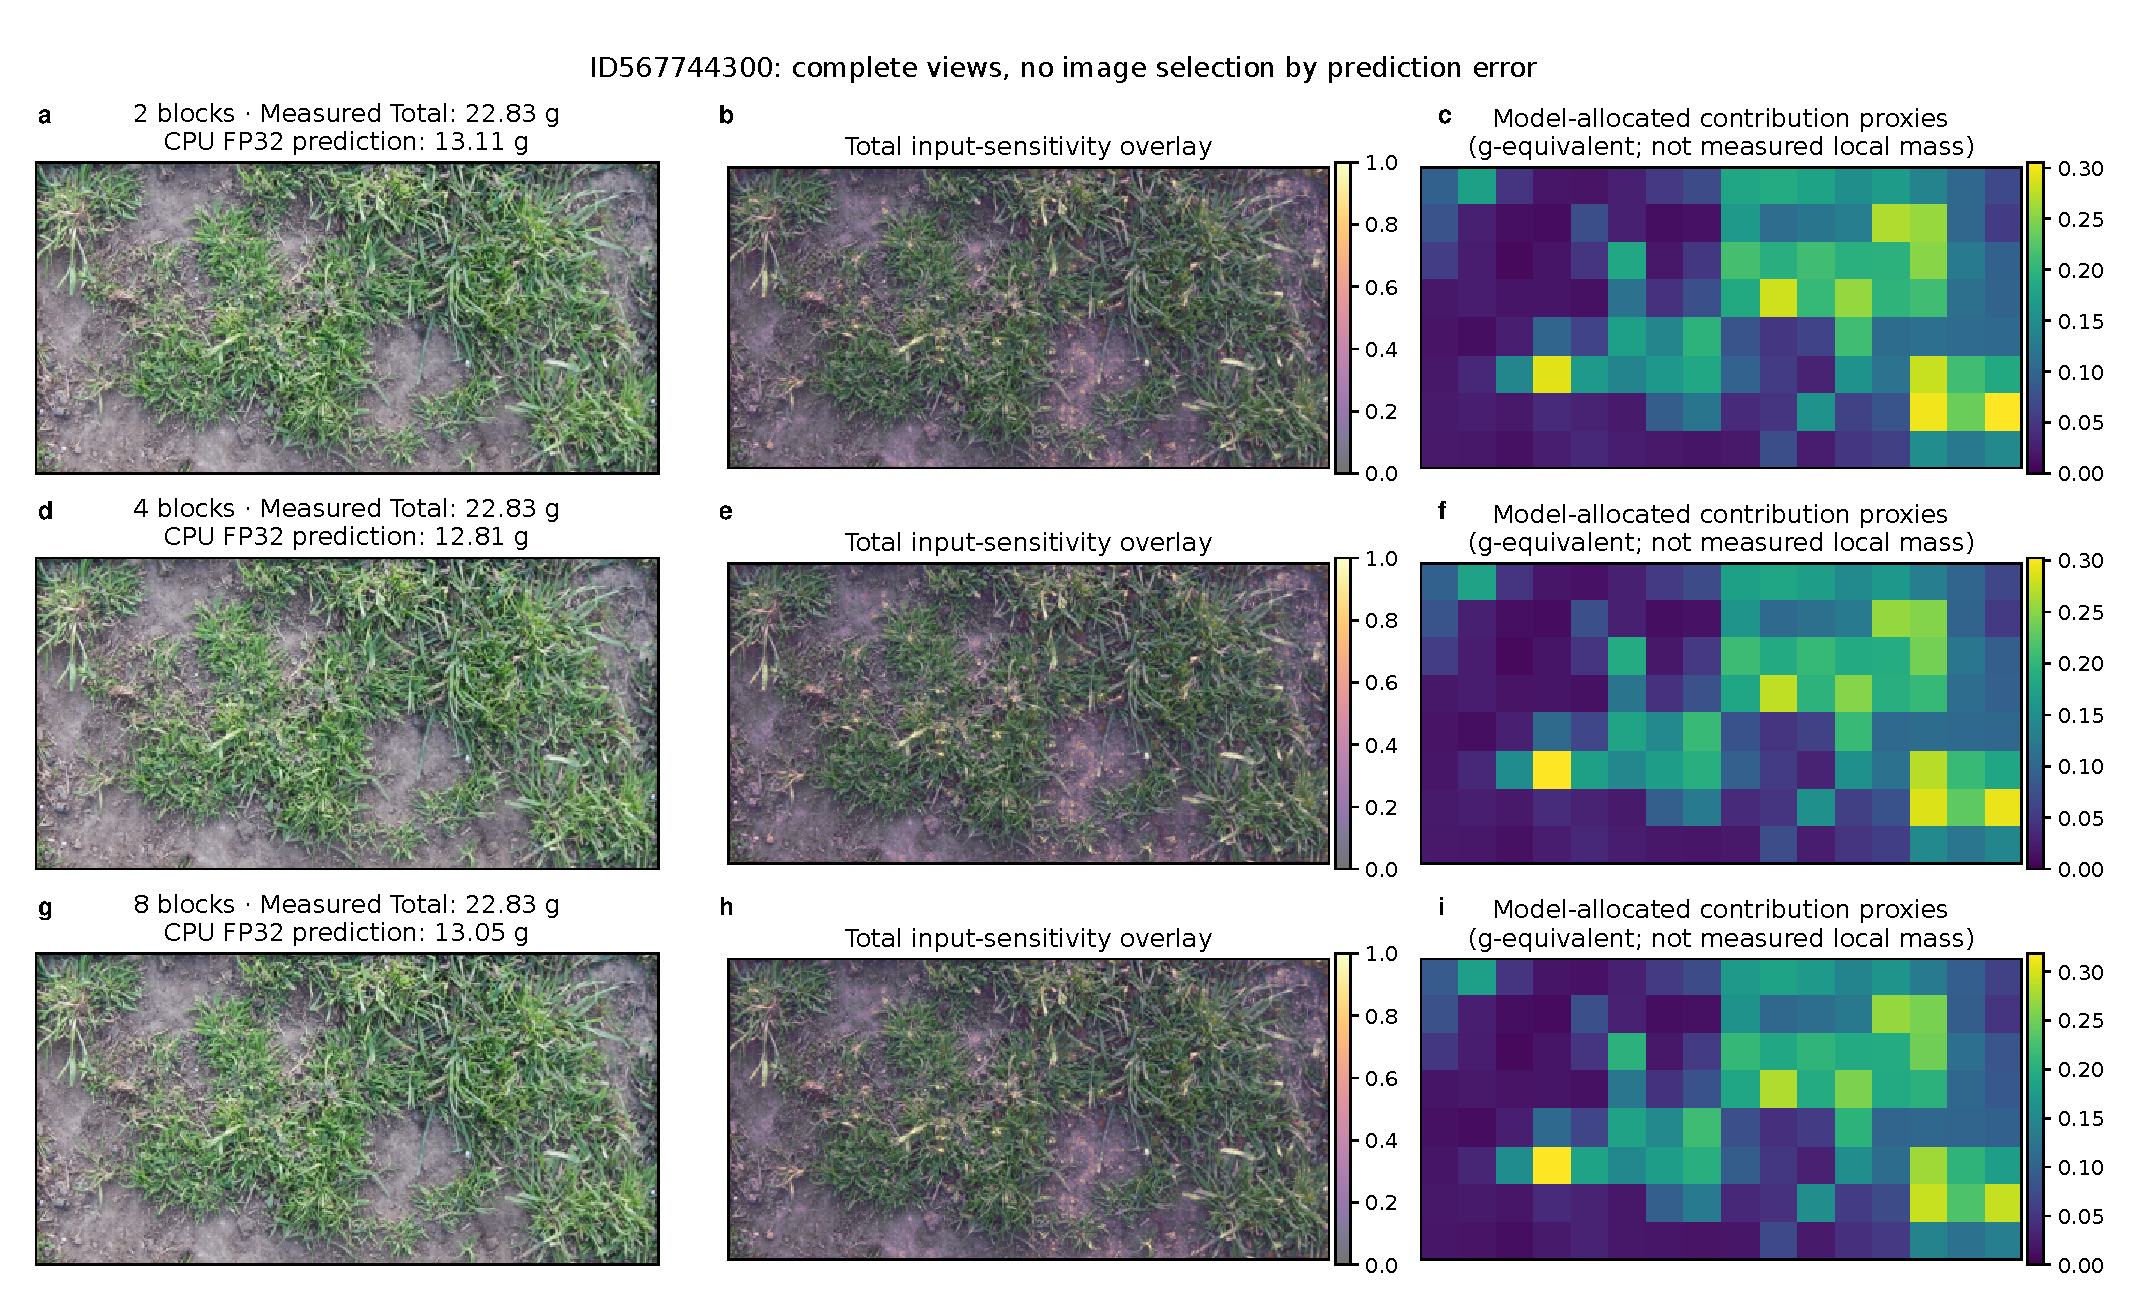
\includegraphics[width=\linewidth,height=.72\textheight,keepaspectratio]{figures/ID567744300_depth_comparison_overlays.pdf}
\caption{Complete DINOv3 sensitivity comparisons for ID567744300, across depths two, four and eight. Each heatmap is separately normalized at its 99th percentile; color intensity is not comparable between models. The contribution grids are model-derived proxies, not measured local biomass.}
\label{fig:s4}
\end{figure}
\begin{figure}[!htbp]
\centering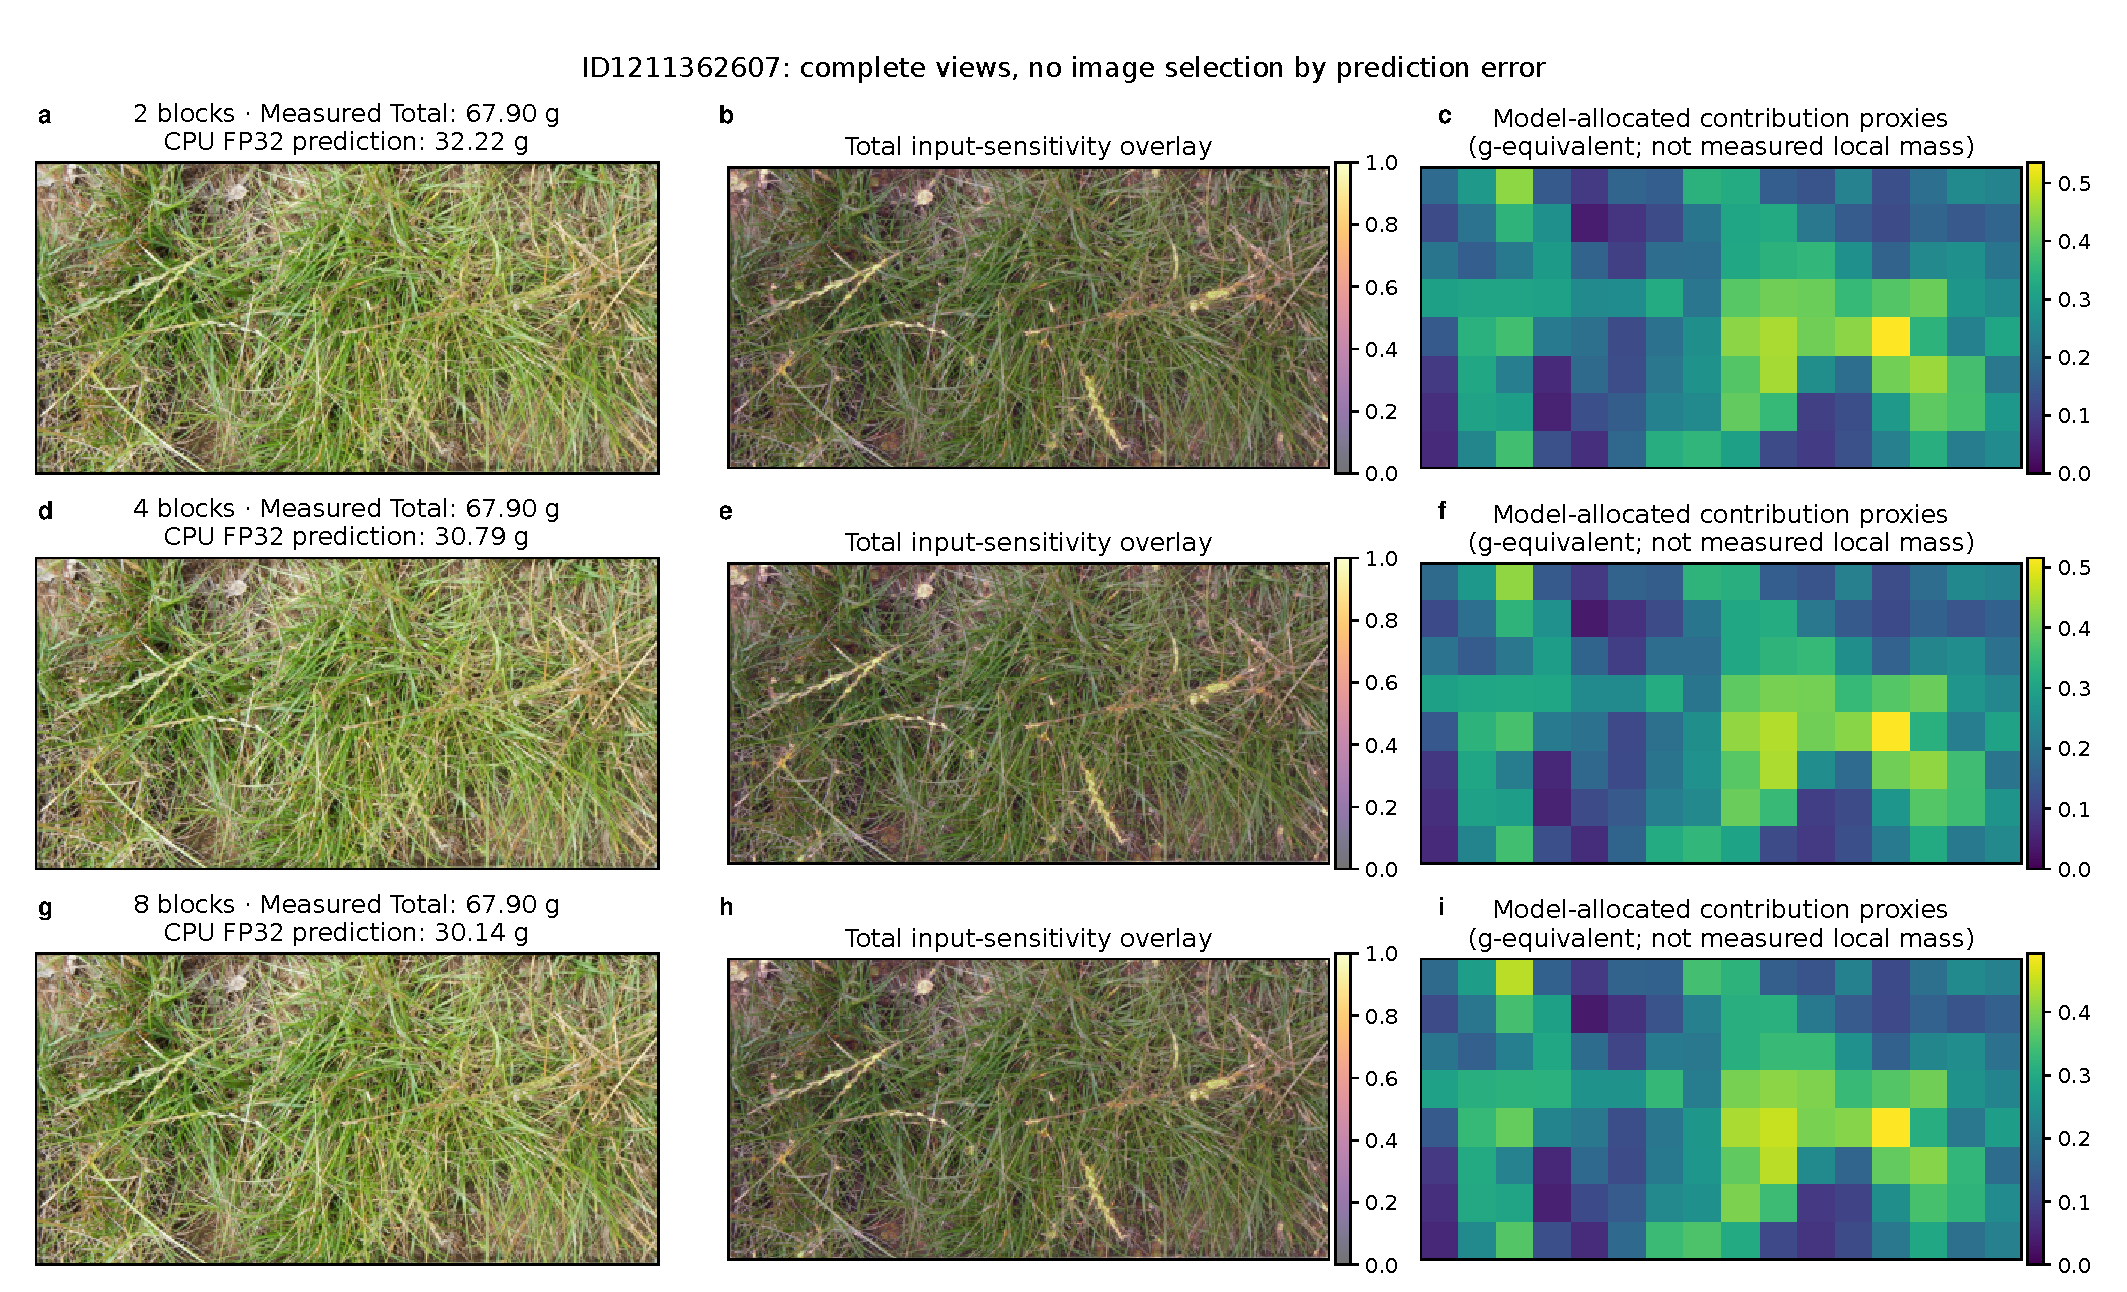
\includegraphics[width=\linewidth,height=.72\textheight,keepaspectratio]{figures/ID1211362607_depth_comparison_overlays.pdf}
\caption{Complete DINOv3 sensitivity comparisons for ID1211362607, across depths two, four and eight. Each heatmap is separately normalized at its 99th percentile; color intensity is not comparable between models. The contribution grids are model-derived proxies, not measured local biomass.}
\label{fig:s5}
\end{figure}
\begin{figure}[!htbp]
\centering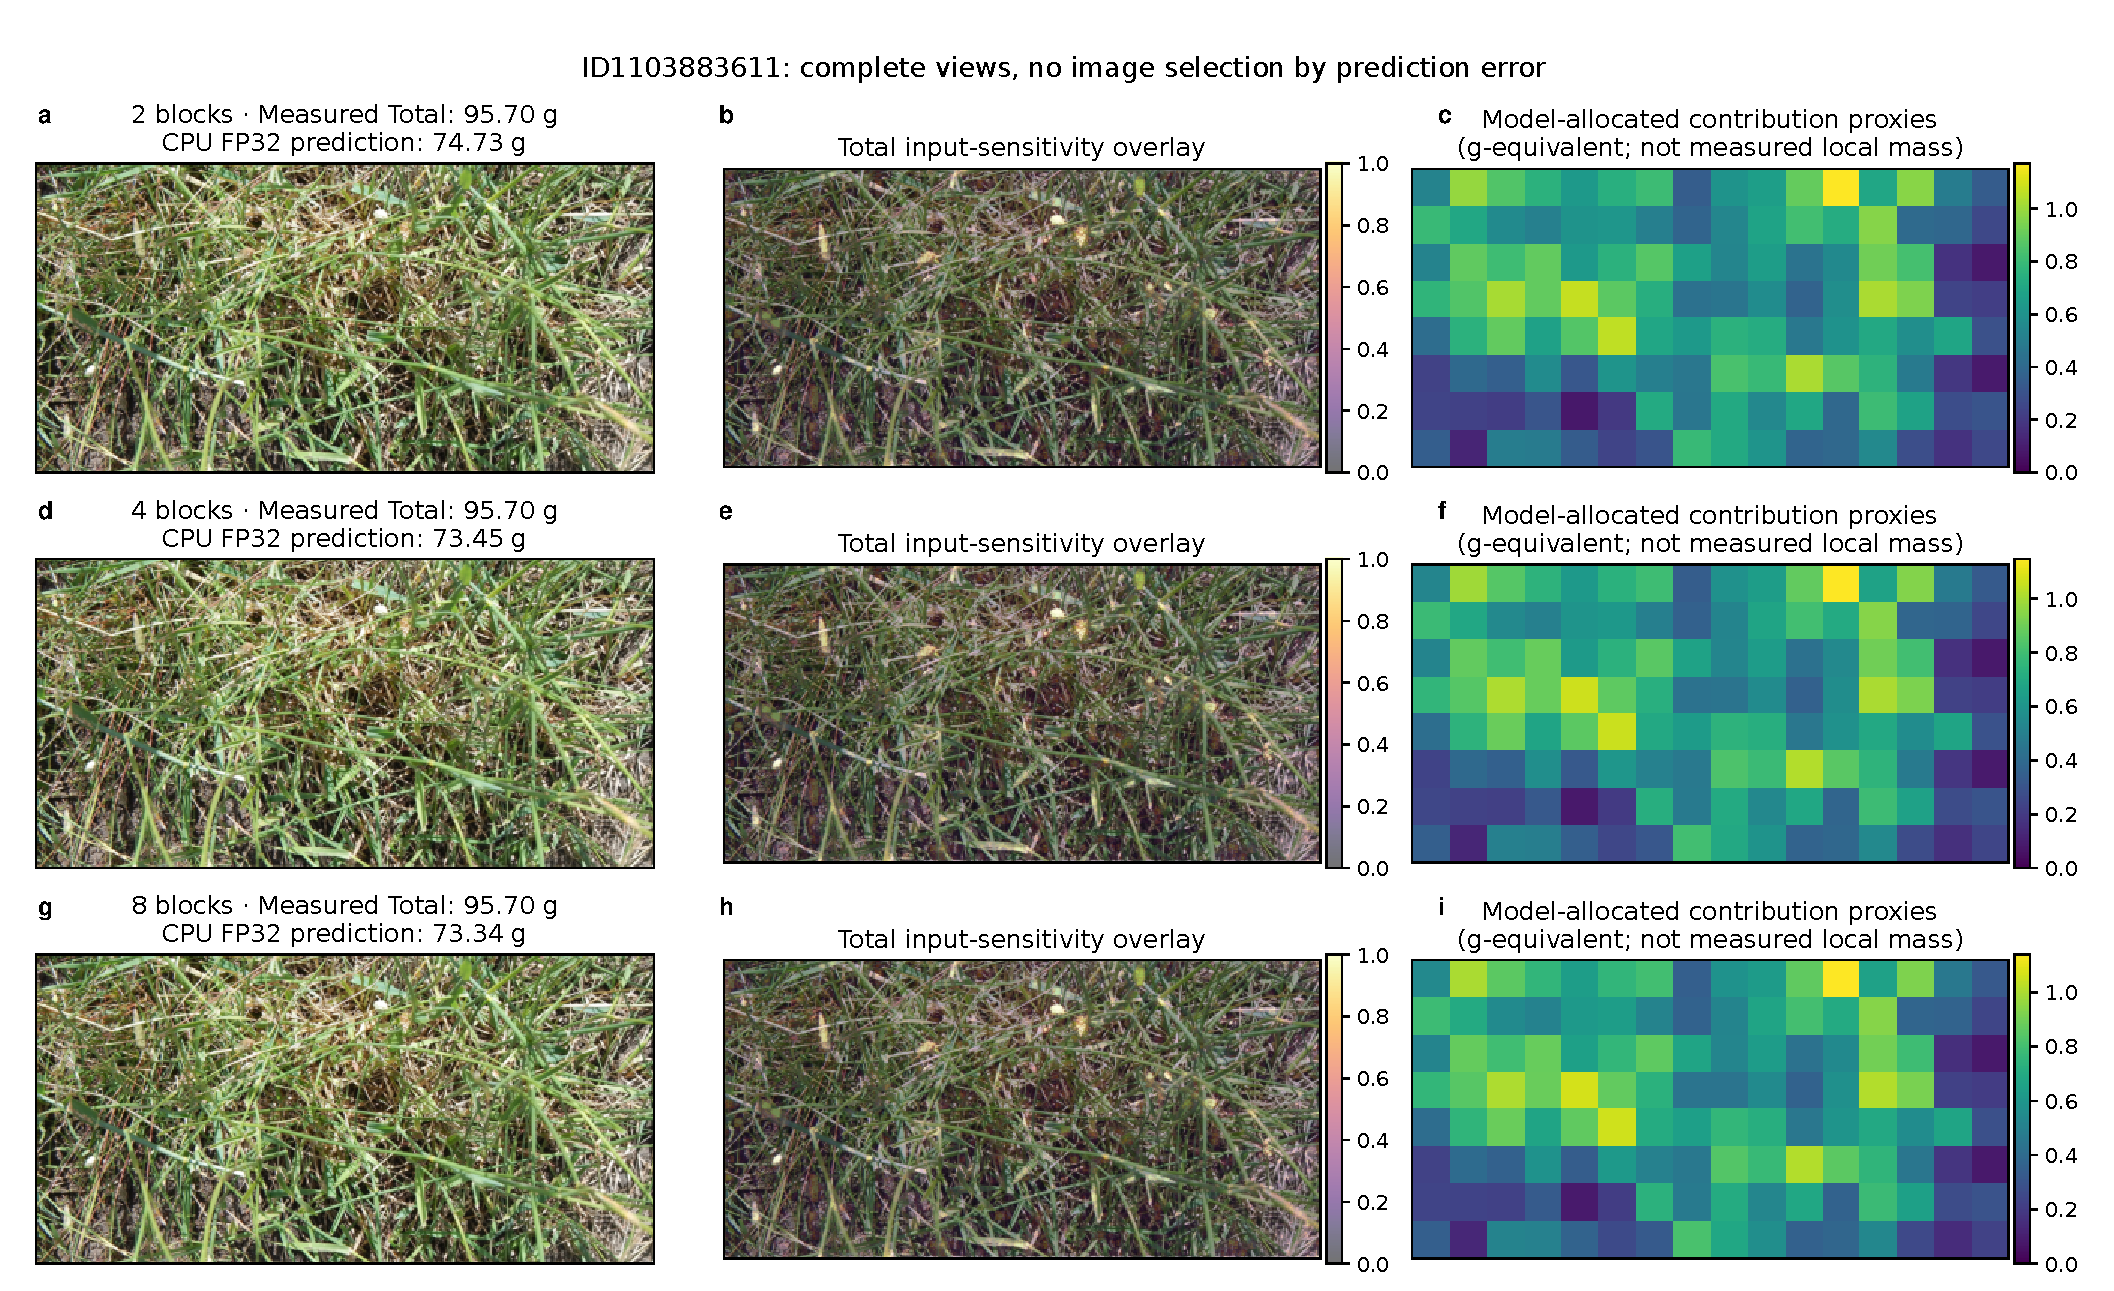
\includegraphics[width=\linewidth,height=.72\textheight,keepaspectratio]{figures/ID1103883611_depth_comparison_overlays.pdf}
\caption{Complete DINOv3 sensitivity comparisons for ID1103883611, across depths two, four and eight. Each heatmap is separately normalized at its 99th percentile; color intensity is not comparable between models. The contribution grids are model-derived proxies, not measured local biomass.}
\label{fig:s6}
\end{figure}
\begin{figure}[!htbp]
\centering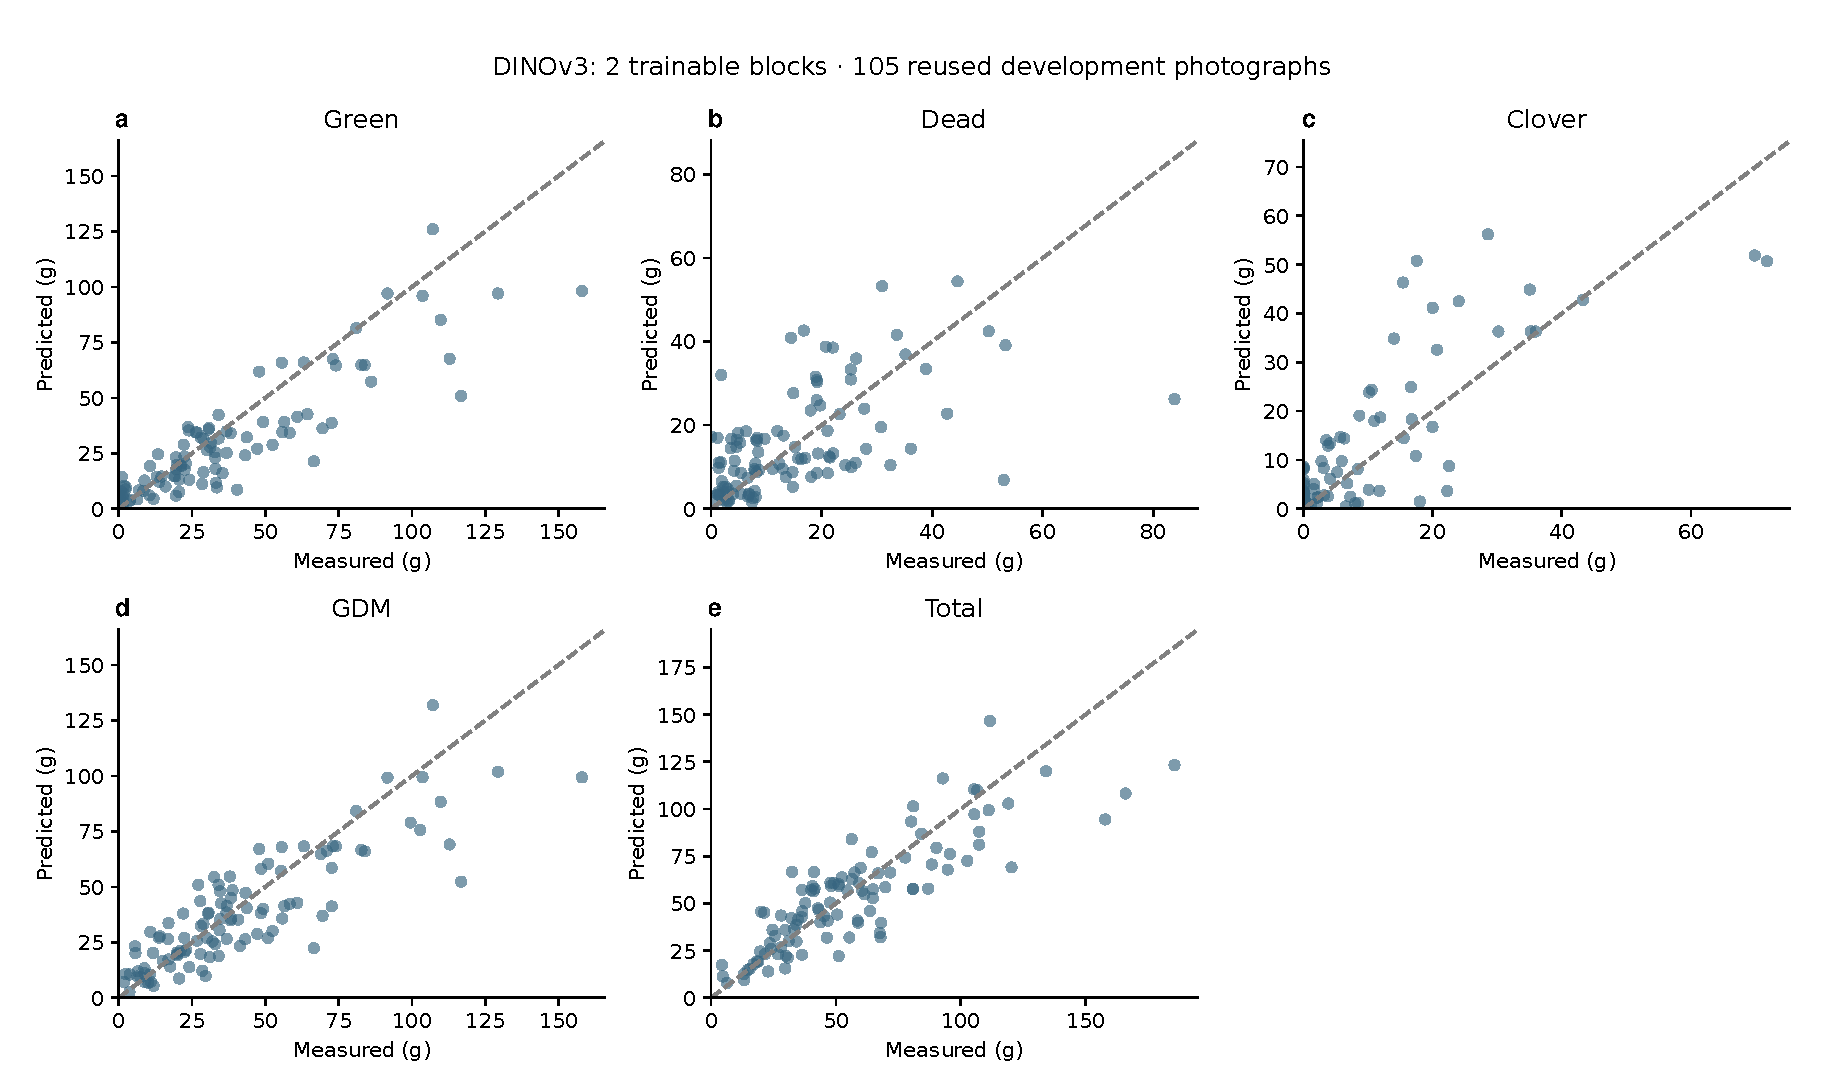
\includegraphics[width=\linewidth,height=.72\textheight,keepaspectratio]{figures/depth_2_all_target_scatter.pdf}
\caption{Measured versus predicted values for all five biomass targets at depth 2. All 105 photographs belong to the repeatedly evaluated development subset; dashed lines indicate equal measured and predicted values.}
\label{fig:s7}
\end{figure}
\begin{figure}[!htbp]
\centering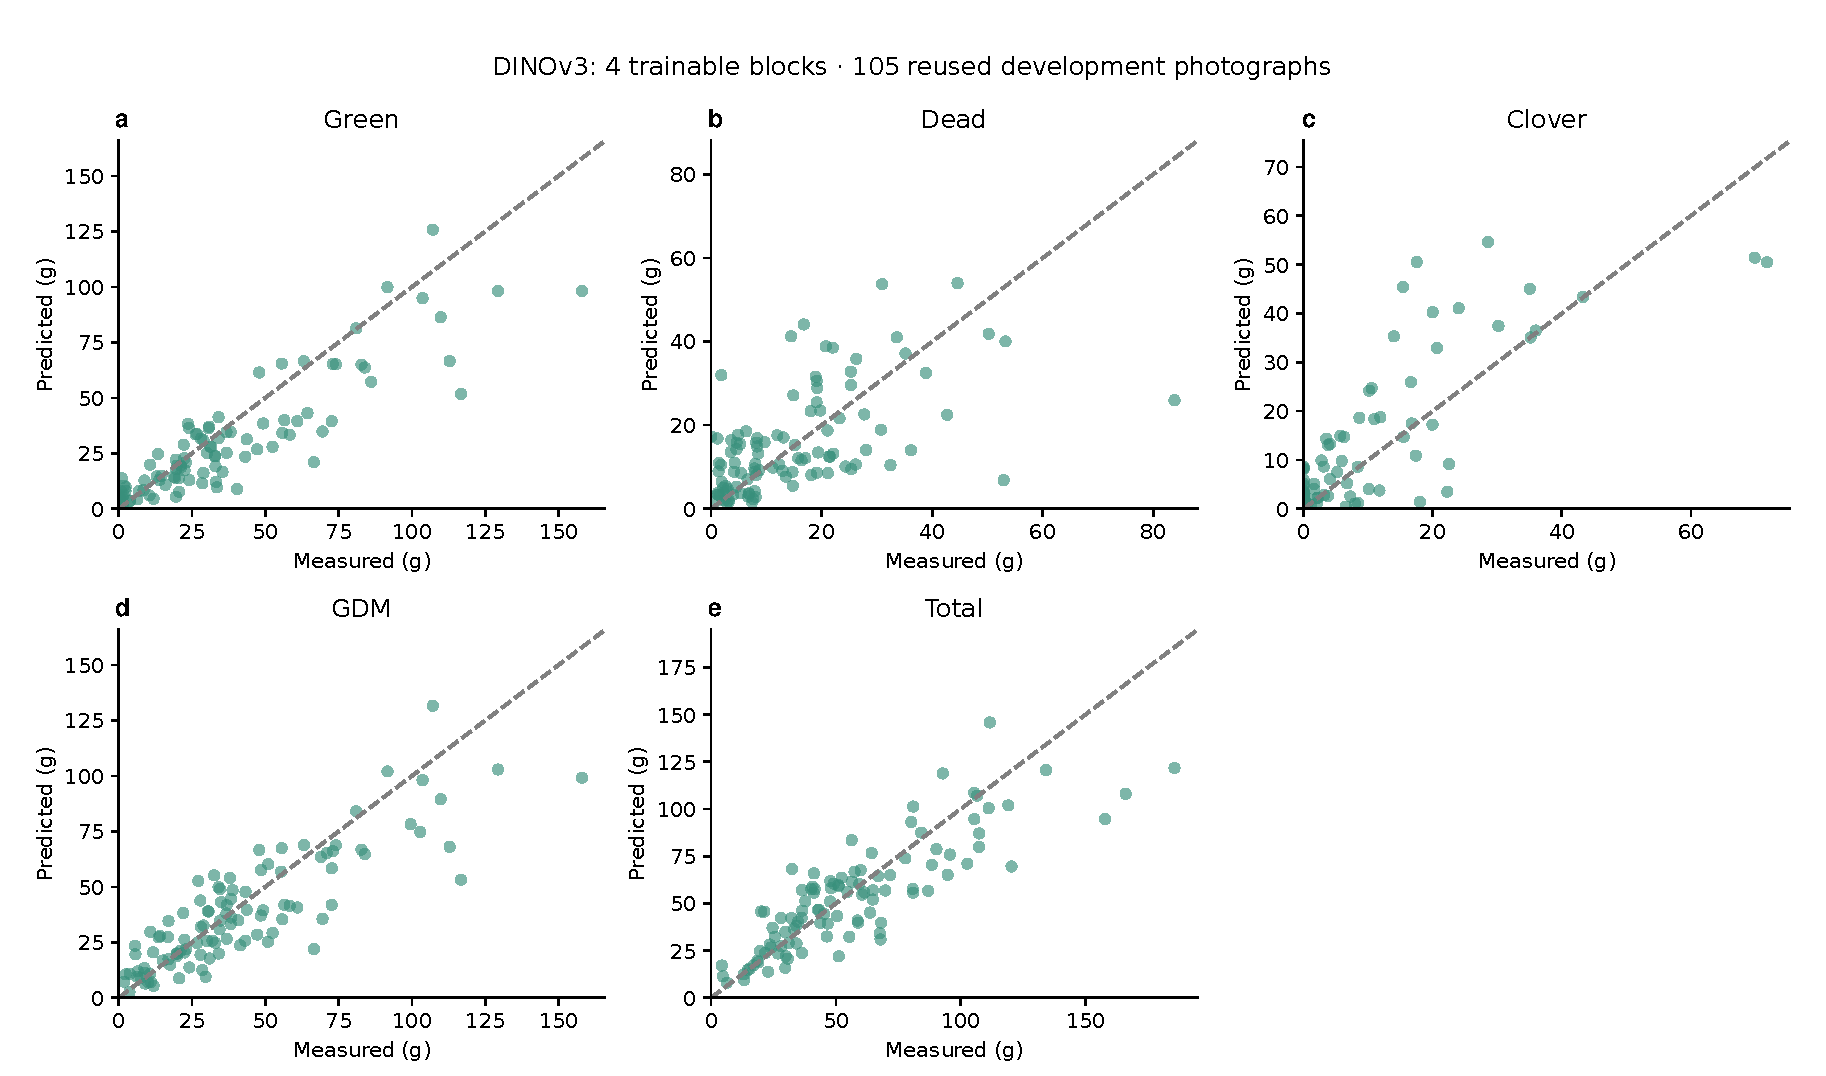
\includegraphics[width=\linewidth,height=.72\textheight,keepaspectratio]{figures/depth_4_all_target_scatter.pdf}
\caption{Measured versus predicted values for all five biomass targets at depth 4. All 105 photographs belong to the repeatedly evaluated development subset; dashed lines indicate equal measured and predicted values.}
\label{fig:s8}
\end{figure}
\begin{figure}[!htbp]
\centering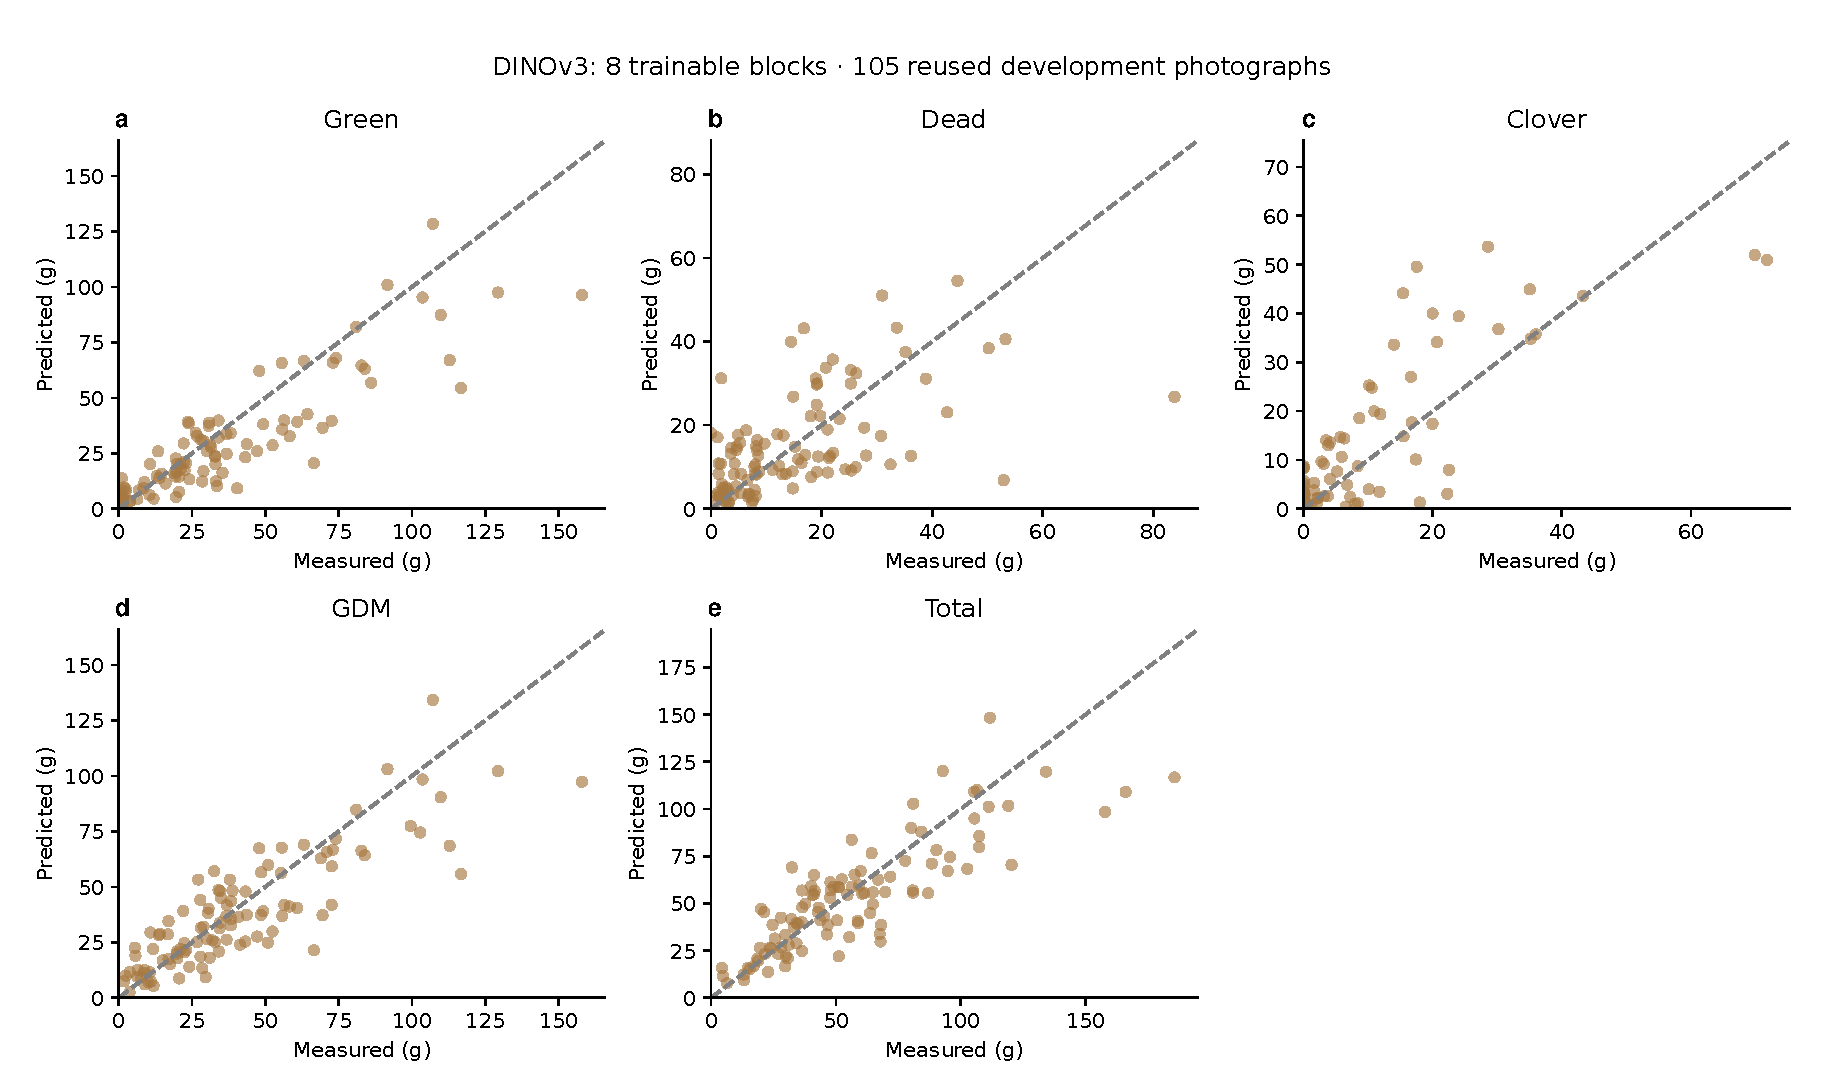
\includegraphics[width=\linewidth,height=.72\textheight,keepaspectratio]{figures/depth_8_all_target_scatter.pdf}
\caption{Measured versus predicted values for all five biomass targets at depth 8. All 105 photographs belong to the repeatedly evaluated development subset; dashed lines indicate equal measured and predicted values.}
\label{fig:s9}
\end{figure}
\begin{figure}[!htbp]
\centering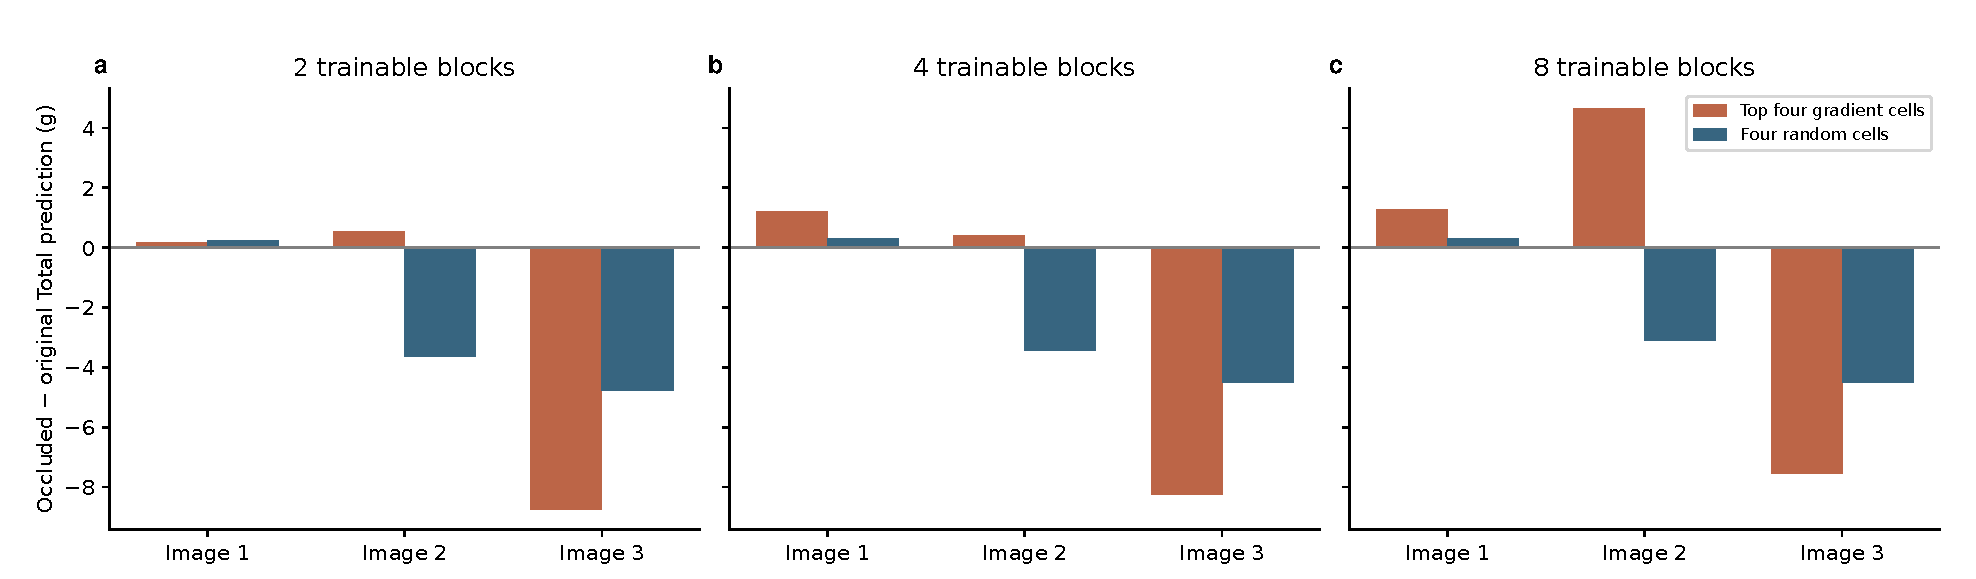
\includegraphics[width=\linewidth]{figures/occlusion_comparison.pdf}
\caption{Finite occlusion diagnostics for all nine DINOv3 model--image combinations. The ordinate is the change in Total prediction after replacing four gradient-ranked or four random cells with mean RGB. The magnitude was greater for gradient-ranked cells in six of nine model--image comparisons; cases are correlated across depths; signed effects show that removing selected regions can either increase or decrease predictions. These artificial interventions are sensitivity checks, not causal or biological validation.}
\label{fig:occlusion}
\label{fig:s10}
\end{figure}
\begin{figure}[!htbp]\centering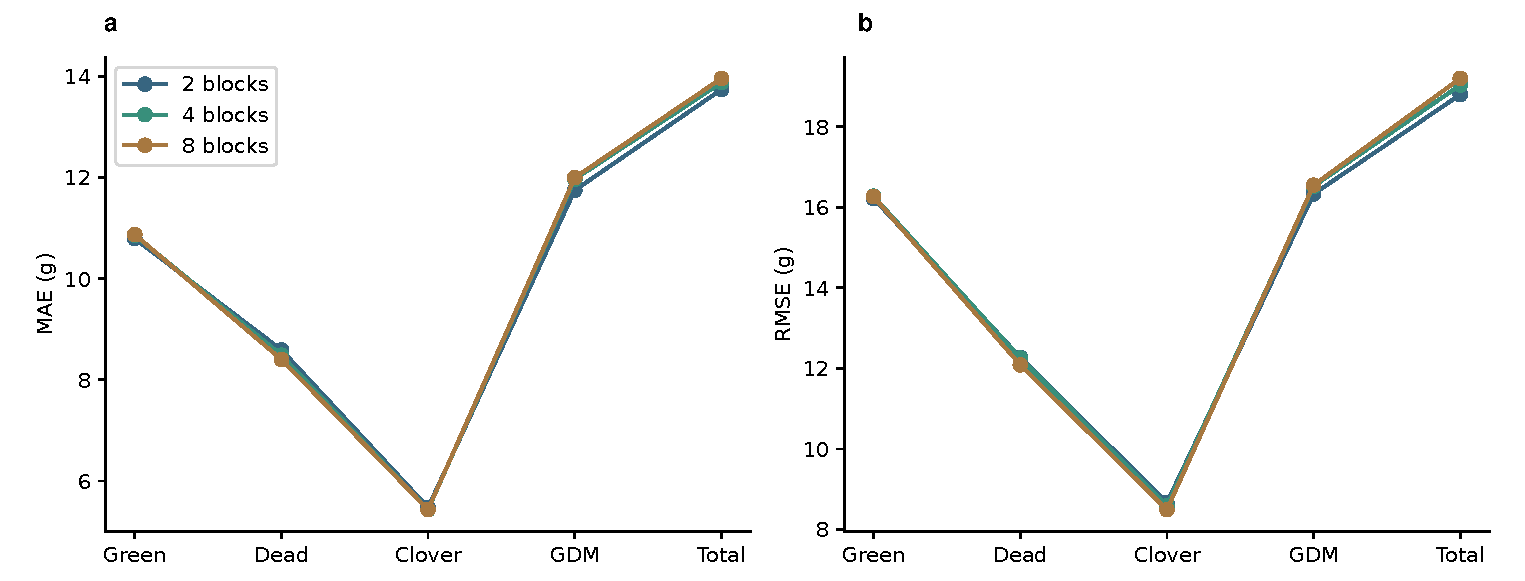
\includegraphics[width=\linewidth]{figures/all_target_errors.pdf}\caption{Per-target MAE and RMSE across fine-tuning depths (2, 4 and 8 blocks), retained as descriptive supplementary analysis.}
\label{fig:s11}
\end{figure}
\end{document}
